\documentclass[handout]{beamer}
\usetheme{PaloAlto}         %controls the width of the sidebar

\usepackage{listings}

% COLORS
\usepackage{color}

\definecolor{Blue}{HTML}{264653}
\definecolor{Green}{HTML}{2a9d8f}
\definecolor{Yellow}{HTML}{e9c46a}
\definecolor{Orange}{HTML}{f4a261}
\definecolor{Red}{HTML}{e76f51}
\definecolor{Black}{HTML}{50514F}

\hypersetup{
    colorlinks=true,
    linkcolor=Blue,
    filecolor=magenta,      
    urlcolor=Blue,
    pdftitle={Sharelatex Example},
    bookmarks=true,
    pdfpagemode=FullScreen,
}

% set colors and layout
\setbeamercolor{frametitle}{bg=Green}     %controls the color of the headline
\setbeamercolor{title}{bg=Blue}		%controls color title bar
\setbeamercolor{sidebar}{bg=Yellow}        %controls the color of the sidebar
\setbeamercolor{logo}{bg=Green}  %controls the color of the logo area
\setbeamercolor{block title}{bg=Orange,fg=black}
\setbeamertemplate{itemize item}[circle]
\setbeamertemplate{itemize subitem}[triangle]
\setbeamertemplate{enumerate items}[default]

\setbeamercolor*{enumerate item}{fg=Blue}
\setbeamercolor{itemize item}{fg=Blue}
\setbeamercolor{itemize subitem}{fg=Green}
\setbeamercolor{navigation symbols}{fg=Green, bg=Blue}
\setbeamercolor{palette sidebar secondary}{fg=black}
\setbeamercolor{section in sidebar shaded}{fg=black}
\setbeamercolor{subsection in sidebar shaded}{fg=black}
\setbeamercolor{author in sidebar}{fg=black}
\setbeamercolor{title in sidebar}{fg=black}
\setbeamercolor{alerted text}{fg=Red}

\setbeamercolor{itemize item}{fg=Blue}
\setbeamercolor{itemize subitem}{fg=Green}
\setbeamercolor{navigation symbols}{fg=Green, bg=Blue}
\setbeamercolor{palette sidebar secondary}{fg=black}
\setbeamercolor{section in sidebar shaded}{fg=black}
\setbeamercolor{subsection in sidebar shaded}{fg=black}
\setbeamercolor{author in sidebar}{fg=black}
\setbeamercolor{title in sidebar}{fg=black}

% remove shadows
\setbeamertemplate{blocks}[rounded]% [shadow=false]
\setbeamertemplate{title page}[default][colsep=-4bp,rounded=true]


\addtobeamertemplate{navigation symbols}{}{%
    \usebeamerfont{footline}%
    \usebeamercolor[fg]{footline}%
    \hspace{1em}%
    \insertframenumber/\inserttotalframenumber
}

% PRESENTATION DETAILS

\title[BWD 2018-2019]{Oefeningen Biowiskundedagen\\Editie 2018-2019}
\author[Michiel, An, Micha\"el]{Michiel Stock\\An Schelfaut\\Michael Ghijs}
\date{5 en 7 februari 2019}
%\logo{\includegraphics[height=1.2cm]{IMG}}
%\institute[VFU] % (optional)

%\makeatletter
%\beamer@headheight=1.5\baselineskip     %controls the height of the headline, default is 2.5    
%\makeatother

\begin{document}
\frame{\titlepage}
\section{Jupyter notebooks}

\section{Secundaire structuurbepaling}

\subsection{Blauwkoorts en groenzucht}

\begin{frame}{Blauwkoorts en groenzucht}
\pause
$$
P(\text{blauwkoorts}) = 0.8\quad\quad P(\text{groenzucht}) = 0.2
$$
\pause
\begin{center}
   \begin{tabular}{lcc} % Column formatting, @{} suppresses leading/trailing space
   \hline \hline
     ziekte      & kans blauw gezicht & kans groen gezicht \\
     \hline
     blauwkoorts & 0.8  & 0.2\\
     groenzucht & 0.3 & 0.7 \\
     \hline \hline
   \end{tabular}
  \end{center}
\pause
$$
P(\text{blauw gezicht}) = 0.8 \times 0.8 + 0.2\time 0.3 =0.7
$$

$$
P(\text{groen gezicht}) = 0.2\times\times 0.8 + 0.7\times0.2=0.3
$$
\pause
$$
P(\text{BK} \mid \text{GG}) =\frac{P( \text{GG}\mid\text{BK})\times P(\text{BK})}{P(\text{GG})}\pause=\frac{0.2\times 0.8}{0.3}\approx0.533
$$
\pause
$$
 P(\text{GZ} \mid \text{GG})  \approx 0.467
$$
\end{frame}

\begin{frame}{Visuele controle}

\subsection{Naive Bayes}

\center{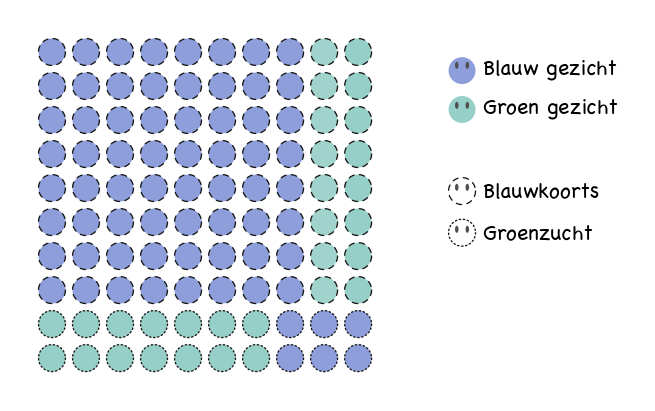
\includegraphics[width=8cm]{../figuren/ziektebayes.png}}

$$
P(\text{BK} \mid \text{GG}) =\frac{16\% \text{ groen gezicht EN blauwkoorts}}{30\% \text{ groen gezicht}} = 0.53
$$
\end{frame}

\begin{frame}{Kansen $\beta$-plaat (1)}
$$
P(\beta\text{-plaat}) = \frac{331}{667} = 0.496
$$
\pause
en de kans op een geen $\beta$-plaat:

$$
P(\text{geen }\beta\text{-plaat}) = \frac{336}{667} = 1 - 0.496 = 0.504
$$

\pause

En dus (vermenigvuldig alle kansen):

\begin{align*}
P(\text{eiwitsequentie} \mid \text{$\beta$-plaat}) &= 0.0181\times 0.0906\times \ldots \\
& \approx 2.98817\times 10^{-9}
\end{align*}
\pause
en

$$
P(\text{seq.} \mid \text{geen }\text{$\beta$-plaat}) = 1.862\times 10^{-11}
$$

\end{frame}

\begin{frame}{Kansen $\beta$-plaat (2)}

\begin{align*}
P(\text{seq.\ en } \text{$\beta$-plaat}) &= P(\text{seq.} \mid \text{$\beta$-plaat}) \times P(\text{$\beta$-plaat}) \\
& \approx 2.98817\times 10^{-9} \times 0.496 = 1.48\times 10^{-9}
\end{align*}

$$
P(\text{seq.\ en } \text{geen $\beta$-plaat}) = 9.38\times 10^{-11}
$$

\pause

Dus:

En dus finaal, volgens de regel van Bayes:

$$
P( \text{$\beta$-plaat} \mid \text{seq.}) \approx \frac{1.48\times 10^{-9}}{1.48\times 10^{-9}+9.38\times 10^{-11}}=0.9404
$$

Het is dus erg waarschijnlijk dat dit deel is van een $\beta$-plaat!

\end{frame}

\begin{frame}{Glijdend venster vragen}
\begin{itemize}
\item grotere $k$ is een langer venster, meer aminozuren worden meegenomen, dus meer zekerheid, wel risico dat je over de grens tussen twee regio's zit
\item $k=1$: slechts \'e\'en aminozuur gebruiken, weinig informatie!
\item hogere drempelwaarde: strenger, minder FP, maar ook meer FN
\item heel hoge drempelwaarde: enkel regio's waar je erg zeker van worden als $\beta$-plaat geclas.\ meer kans dat je er mist.
\end{itemize}
\end{frame}

\section{Ziekteverspr.\ op een netwerk}
\begin{frame}{SIR}
Aantal individuen is constant, want $\frac{\text{d}}{\text{d}t}(S(t) + I(t) +R(t))= 0$:
\begin{multline*}
\frac{\text{d}S(t)}{\text{d}t} + \frac{\text{d}I(t)}{\text{d}t}+ \frac{\text{d}R(t)}{\text{d}t}= -\beta  S(t)  I(t) \\+\beta  S(t) I(t) - \gamma  I(t)+\gamma I(t)=0
\end{multline*}
\end{frame}

\begin{frame}{Verbindingsmatrix voorbeeldnetwerk}
\small
\begin{tabular}{l|rrrrrrrrrrrrrrr}

{} &  1  &  2  &  3  &  4  &  5  &  6  &  7  &  8  &  9  &  10 &  11 &  12 &  13 &  14 &  15 \\
\hline
1  &   0 &   0 &   1 &   1 &   1 &   1 &   0 &   0 &   1 &   0 &   0 &   0 &   0 &   0 &   1 \\
2  &   0 &   0 &   1 &   0 &   0 &   0 &   1 &   0 &   0 &   0 &   0 &   0 &   1 &   0 &   0 \\
3  &   1 &   1 &   0 &   1 &   1 &   1 &   0 &   1 &   1 &   1 &   1 &   1 &   1 &   1 &   0 \\
4  &   1 &   0 &   1 &   0 &   0 &   0 &   1 &   0 &   0 &   0 &   0 &   1 &   0 &   0 &   0 \\
5  &   1 &   0 &   1 &   0 &   0 &   0 &   0 &   0 &   0 &   0 &   0 &   0 &   0 &   0 &   0 \\
6  &   1 &   0 &   1 &   0 &   0 &   0 &   0 &   0 &   0 &   0 &   0 &   0 &   0 &   0 &   0 \\
7  &   0 &   1 &   0 &   1 &   0 &   0 &   0 &   1 &   0 &   0 &   0 &   0 &   0 &   0 &   0 \\
8  &   0 &   0 &   1 &   0 &   0 &   0 &   1 &   0 &   0 &   1 &   1 &   0 &   0 &   1 &   0 \\
9  &   1 &   0 &   1 &   0 &   0 &   0 &   0 &   0 &   0 &   0 &   0 &   0 &   0 &   0 &   1 \\
10 &   0 &   0 &   1 &   0 &   0 &   0 &   0 &   1 &   0 &   0 &   0 &   0 &   0 &   0 &   0 \\
11 &   0 &   0 &   1 &   0 &   0 &   0 &   0 &   1 &   0 &   0 &   0 &   0 &   0 &   0 &   0 \\
12 &   0 &   0 &   1 &   1 &   0 &   0 &   0 &   0 &   0 &   0 &   0 &   0 &   0 &   0 &   0 \\
13 &   0 &   1 &   1 &   0 &   0 &   0 &   0 &   0 &   0 &   0 &   0 &   0 &   0 &   0 &   0 \\
14 &   0 &   0 &   1 &   0 &   0 &   0 &   0 &   1 &   0 &   0 &   0 &   0 &   0 &   0 &   0 \\
15 &   1 &   0 &   0 &   0 &   0 &   0 &   0 &   0 &   1 &   0 &   0 &   0 &   0 &   0 &   0 \\

\end{tabular}
\end{frame}

\end{document}